% Preamble
\documentclass[12pt]{article}

% Packages
\usepackage[left=3.0cm, right=1.5cm, top=2.0cm, bottom=2.0cm]{geometry}

\usepackage[utf8]{inputenc}
\usepackage[T2A]{fontenc}
\usepackage[russian]{babel}
\usepackage{amsmath, amsfonts, amssymb}
\usepackage{graphicx}
\usepackage{wrapfig}
\usepackage{fancyhdr}
\usepackage[shortlabels]{enumitem}
\usepackage{svg}
\usepackage{amstex}
\usepackage{colortbl}
\usepackage{bm}
\usepackage{amsfonts}
\usepackage{amssymb}

\renewcommand{\vec}{\textbf}
\newcommand{\cross}{\times}

\pagestyle{fancy}
\fancyhead[L]{Работа №4.3.1}
\fancyhead[R]{Белинский Т.Д.\quad Б05-206}

% Document
\begin{document}
    \section*{4.3.1. ИЗУЧЕНИЕ ДИФРАКЦИИ СВЕТА}
    \ \par
    \textbf{Цель работы:} Цель работы: исследовать явления дифракции Френеля и Фраунгофера на одной и двух
    щелях, изучить влияние дифракции на разрешающую способность оптических инструментов;
    проверить теоретические соотношения для положения максимумов при дифракции Френеля
    и Фраунгофера.

    \textbf{Оборудование:} оптическая скамья, ртутная лампа, светофильтр,
    щели с регулируемой шириной, рамка с вертикальной нитью, экран с двойной щелью,
    микроскоп на поперечных салазках с микрометрическим винтом, зрительная труба.

    \subsection*{Теоретическая часть}
    \subsection*{A. Дифракция Френеля}
    \ \par
    \begin{figure}[h]
        \centering
        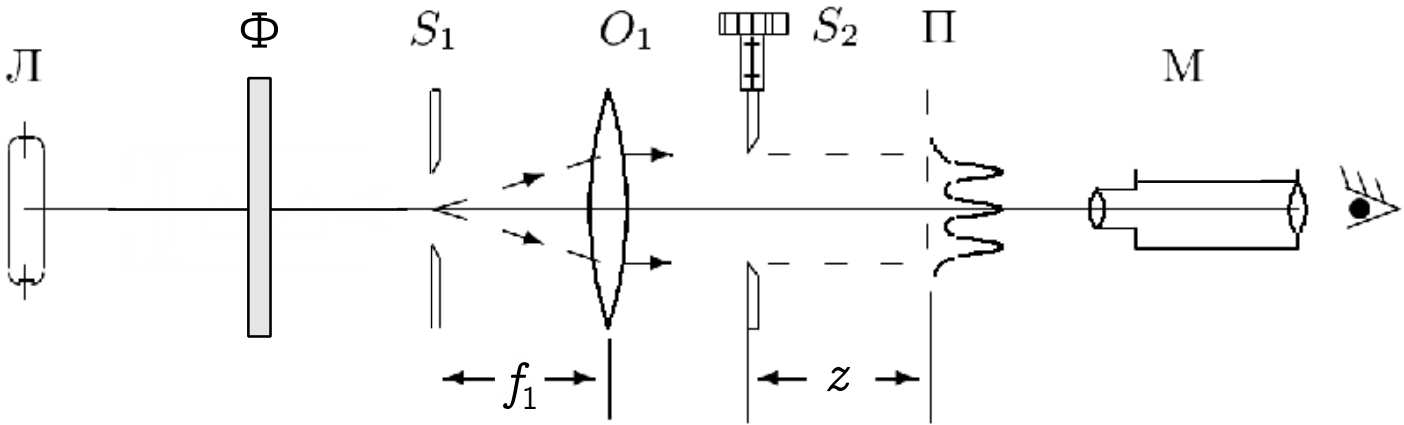
\includegraphics[width=\linewidth]{pic/setupA}
        \caption{Схема установки для наблюдения дифракции Френеля}
        \label{fig:1}
    \end{figure}
    Схема установки для наблюдения дифракции Френеля представлена на\ \figurename{\ref{fig:1}} Свет
    от ртутной ртутной ламы Л, пропущенный через оранжевый светофильтр Ф со средней
    длиной волны $\lambda = 578$ нм, падает на входную щель $s_1$.
    Щель $s_1$ находится в фокусе коллиматора — собирающей линзы $O_1$.
    Коллиматор создаёт параллельный пучок монохроматического света, освещающий щель $s_2$,
    на которой и происходит дифракция.
    Дифракционная картина рассматривается с помощью микроскопа M, сфокусированного на
    некоторую плоскость наблюдения П.

    Распределение интенсивности света в плоскости наблюдения П проще всего рассчитывать с помощью зон Френеля
    (для щели их также называют зонами Шустера).
    При освещении щели $s_2$ параллельным пучком лучей (плоская волна) зоны Френеля представляют собой полоски,
    параллельные краям щели.
    Результирующая амплитуда в точке наблюдения определяется суперпозицией колебаний от тех зон Френеля,
    которые не перекрыты створками щели.
    Границы зон Френеля/Шустера $\xi_m$ определяется соотношением
    \begin{equation}
        \xi_m \pm \sqrt{mz\lambda},\ m\in \mathbb{N},
        \label{eq:1}
    \end{equation}
    где $\xi$ отсчитывается от центра щели, $z$ -- расстояние от щели до плоскости наблюдения П,
    а $\lambda$ — длина волны.
    При ширине щели $b$ $(-b/2 < \xi < b/2)$ полное число открытых зон для
    точки наблюдения на оси равно
    \[
        m_{max} = \frac{b^2}{4\lambda z}.
    \]

    По определению, разделение волнового фронта на зоны Френеля
    производится так, чтобы излучение от соседних зоны находилось в противофазе.
    Иными словами, разность хода (от поверхности фронта до точки наблюдения) между краями соседних зон равна $\lambda/2$.
    Поэтому, когда открыто чётное число зон Френеля, на оси системы наблюдается минимум дифракционной картины (тёмная полоса).
    Если число открытых зон нечётно, в центре картины — максимум (светлая полоса).

    Зафиксируем размер щели $b$ и проанализируем, как меняется картина в зависимости от расстояния до плоскости наблюдения $z$.
    Если число открытых зон Френеля велико, $m \gg 1 (z \rightarrow 0)$, мы приходим к пределу геометрической оптики.
    В нём дифракционная картина отсутствует, а размер изображения щели совпадает с шириной самой щели $b$.
    Дифракционная картина наблюдается только в узкой полосе вблизи границ щели («дифракция на краю экрана»).
    При удалении от плоскости геометрического изображения эти две группы полос
    постепенно расширяются, заполняя всё изображение щели.
    При $m \sim 1$ на щели наблюдается сложная картина из небольшого числа дифракционных полос.
    При дальнейшем удалении $(m \ll 1, z \rightarrow \infty)$ дифракционная картина начинает упрощаться и расширяться,
    переходя в режим Фраунгофера — затухающие по интенсивности эквидистантные полосы
    с характерным угловым размером центральной полосы $\lambda/b$.

    Амплитуду света в произвольной точке плоскости наблюдения можно определить графически с помощью векторной диаграммы — спирали Корню.

    Распределение амплитуд в режиме дифракции Френеля $(m \sim 1)$ довольно сложно.
    Однако если число открытых зон Френеля больше единицы и близко к целому $m = 2, 3, 4, \dots$,
    то в картине можно довольно чётко выделить $m - 1$ тёмных полос, заполняющих изображение щели.
    Так можно по виду дифракционной картины оценить число зон Френеля на полуширине щели.

    \subsection*{Б. Дифракция Фраунгофера на щели}
    \ \par
    \begin{figure}[h]
        \centering
        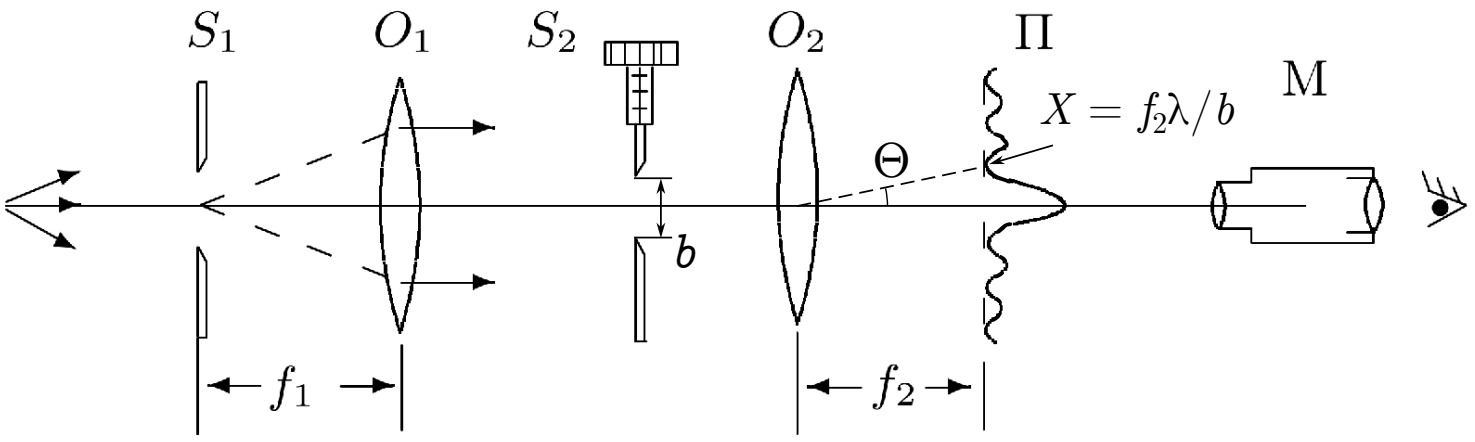
\includegraphics[width=\linewidth]{pic/setupB}
        \caption{Схема установки для наблюдения дифракции Фраунгофера на щели}
        \label{fig:2}
    \end{figure}
    На значительном удалении от щели, когда выполнено условие $m \ll 1$ (то есть ширина
    щели становится значительно меньше ширины первой зоны Френеля, $(b\ll\sqrt{\lambda z})$,
    изображение щели размывается и возникает дифракционная картина, называемая дифракцией Фраунгофера.
    Дифракцию Фраунгофера можно наблюдать той же установке, что и дифракцию Френеля\ \figurename{\ref{fig:1}}.
    Однако при обычных размерах установки дифракция Фраунгофера возникает только при очень узких щелях.
    Поскольку работать с тонкими щелями неудобно, длянаблюдения дифракции Фраунгофера к схеме добавляется объектив $O_2$\ \figurename{\ref{fig:2}}.

    Дифракционная картина наблюдается в фокальной плоскости объектива $O_2$.
    Поскольку объектив не вносит дополнительной разности хода между интерферирующими лучами
    (таутохронизм тонкой линзы), в его фокальной плоскости наблюдается неискажённая
    дифракционная картина Фраунгофера, соответствующая бесконечно удалённой плоскости наблюдения.
    При дифракции Фраунгофера в центре поля зрения наблюдается дифракционный максимум (светлая полоса).
    Сбоку от неё наблюдаются чередующиеся минимумы и максимумы с довольно быстро затухающей интенсивностью.
    Направление на минимумы (тёмные полосы) при малых углах $\theta$ определяется соотношением
    \begin{equation}
        \theta^{min}_n=n\frac{\lambda}{b},\ n=\pm1,\pm2,\dots,
        \label{eq:2}
    \end{equation}
    где $b$ -- ширина щели.
    Каждому значению угла $\theta$ соответствует точка в плоскости объектива с фокусным расстоянием $f_2$,
    отстоящая от оптической оси на расстоянии
    \begin{equation}
        X_n = f_2 \tan \theta_n \approx f_2 \theta_n.
        \label{eq:3}
    \end{equation}
    Измеряя зависимость $X$ от $m$ или расстояние между полосами $\DeltaX$, можно определить
    ширину щели $s_2$.

    \subsection*{В. Дифракция Фраунгофера на двух щелях}
    \ \par
    \begin{figure}[h]
        \centering
        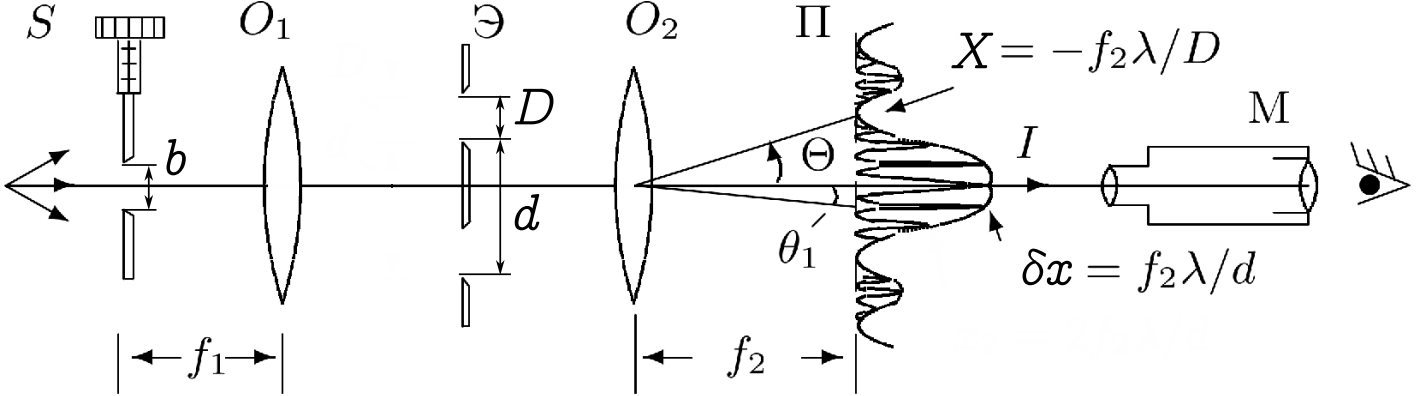
\includegraphics[width=\linewidth]{pic/setupC}
        \caption{Схема установки для наблюдения дифракции Фраунгофера на двух щелях}
        \label{fig:3}
    \end{figure}
    Схема для наблюдения дифракции Фраунгофера на двух щелях изображена на\ \figurename{\ref{fig:3}}
    По сравнению с\ \figurename{\ref{fig:2}} в ней щель $s_2$ заменена на экран Э с двумя щелями.
    При этом щель $s_2$ (с микрометрическим винтом) установлена вместо входной щели $s_1$ (для измерения
    влияния ширины источника на чёткость картины).

    Результат дифракции на двух щелях можно представить как интерференцию дифракционных картин от каждой щели (аналог интерференционной схемы Юнга)

    Если входная щель достаточно узка, то дифракционная картина в плоскости П (\figurename{\ref{fig:3}})
    подобна той, что получалась при дифракции на одной щели, однако теперь вся картина
    испещрена рядом дополнительных узких полос.
    Наличие этих полос объясняется суперпозицией (интерференцией) световых волн,
    приходящих в плоскость наблюдения через разные щели экрана Э.
    В центре главного дифракционного максимума располагается светлая полоса (разность на оси, в силу симметрии, равна нулю).
    Светлая интерференционная полоса наблюдается также, когда разность хода кратна длине волны.
    Угловая координата $\theta_n$ интерференционного максимума $n$-го порядка определяется соотношением
    \begin{equation}
        \theta_n d = n\lambda,\ n = \pm1, \pm2,\dots
        \label{eq:4}
    \end{equation}
    где $d$ -- расстояние между щелями.
    Линейное расстояние $\delta x$ между соседними интерференционными полосами в плоскости П равно поэтому
    \begin{equation}
        \delta x = f_2 \frac{\lambda}{d}
        \label{eq:5}
    \end{equation}

    На\ \figurename{\ref{fig:3}} показано распределение интенсивности в фокальной плоскости объектива $O_2$.
    Штриховой линией (в увеличенном масштабе) изображено распределение интенсивности
    при дифракции света на одиночной щели.
    Поскольку полная угловая ширина главного дифракционного максимума (от минимума до минимума) равна $2\lambda/D$,
    где $D$ -- ширина отдельной щели, то на нём укладывается $N =2d/D$ тёмных интерференционных полос
    (в центре картины максимум, поэтому светлых полос — на одну больше).

    При дифракции света на двух щелях чёткая система интерференционных полос
    наблюдается только при достаточно узкой ширине входной щели ($s_2$), которую можно рассматривать как протяжённый источник света размером $b$.
    Для наблюдения интерференции необходимо, чтобы расстояние $d$ между щелями не превышало радиуса когерентности
    \begin{equation}
        d \le \rho_{ког} \approx \frac{\lambda}{b}f_1
        \label{eq:6}
    \end{equation}
    Таким образом, по размытию интерференционной картины можно оценить размер источника $b$.
    Этот метод используется в звёздном интерферометре при измерении угловых размеров звёзд.

    \subsection*{Г. Влияние дифракции на разрешающую способность оптического инструмента}
    \ \par
    \begin{figure}[h]
        \centering
        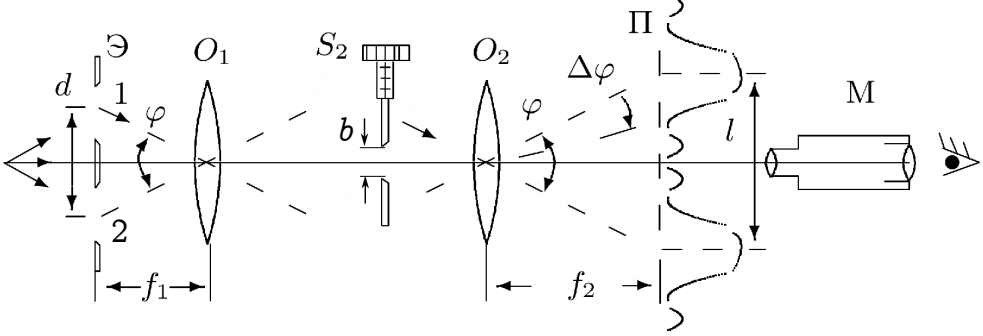
\includegraphics[width=\linewidth]{pic/setupD}
        \caption{Схема установки для исследования разрешающей способности оптического инструмента}
        \label{fig:4}
    \end{figure}
    В качестве предмета будем использовать экран Э с двумя узкими щелями (поместим
    его вместо щели $s_1$). Пусть расстояние между щелями равно $d$. Тогда от каждой из щелей
    экрана на щель $s_2$ будут падать два параллельных пучка света, составляющих между
    собой угол
    \begin{equation}
        \varphi \approx \frac{d}{f_1}
        \label{eq:7}
    \end{equation}
    (а центры двух дифракционных пятен в плоскости П будут находиться на расстоянии
    $l = f_2\varphi$ друг от друга).

    Угловая ширина же $\Delta \varphi$ каждого изображения определяется дифракцией света на щели $s_2$.
    В режиме дифракции Фраунгофера полуширина центрального дифракционного
    максимума равна $\Delta \varphi \sim \lambda/b$, где $b$ -- ширина щели $s_2$.

    Если полуширина главного дифракционного пятна превысит расстояние между центрами пятен $\Delta \varphi > \varphi$,
    пятна от двух щелей сольются в одно, и по виду дифракционной картины будет трудно определить,
    представляет ли собой источник двойную или одиночную щель.
    Это условие разрешения двух изображений называют также критерием Рэлея.
    Итак, щели можно считать различимыми, если
    \begin{equation}
        \frac{\lambda}{b} < \frac{d}{f_1}
        \label{eq:8}
    \end{equation}

    \subsection*{Результаты и обработка}
    \begin{enumerate}
        \item Выставим ширину щели
        \[
            D = (0.312 \pm 0.001)\ \text{мм}.
        \]
        Зависимость количества черных полос $n$ от координаты микроскопа $z$.
        Полученные данные приведены в таблице\ \ref{tab:1}.
        Расстояние от щели до точки наблюдения выражается следующим образом:
        \[
            z = \frac{b^2}{4\lambda m} + z_0,
        \]
        где $z_0$ -- это смещение необходимое, чтобы перевести координату в расстояние до точки наблюдения,
        $m = n + 1$ -- количество зон Френеля, $\lambda = 578$ нм -- длина волны.

        По полученным значениям построили график (рис.\ \ref{fig:5}) и оценим коэффициент наклона:
        \[
            k = (4.6 \pm 0.2)\ \text{см}.
        \]
        По коэффициенту оценим ширину щели:
        \[
            b = \sqrt{k \cdot 4 \lambda} = (0.33 \pm 0.01)\ \text{мм}
        \]

        \item С помощью микроскопа снимаем зависимости координат дифракционных минимумов от номера.
        Полученные данные приведены в таблице\ \ref{tab:2}.
        Координата минимума выражается следующим образом:
        \[
            x_n \approx f_2\frac{\lambda}{b}n,
        \]
        где $f_2=9$ см -- фокусное расстояние линзы.
        По полученным значениям строим график (рис.\ \ref{fig:6}) и оценим коэффициент наклона:
        \[
            k = (0.160 \pm 0.003)\ \text{см}.
        \]
        По коэффициенту оценим ширину щели:
        \[
            b = f_2 \frac{\lambda}{k} = (0.32 \pm 0.01)\ \text{мм}
        \]

        \item Число наблюдаемых темных полос в центральном ``максимуме'' при дифракции Фраунгофера --  $N = 13$.
        Координаты двух самых удаленных темных полос и количество светлых полос между ними:
        \[
            x_1 = (1.02 \pm 0.01)\ \text{мм} \quad x_2 = (1.48 \pm 0.01)\ \text{мм} \quad N_l = 12.
        \]
        Тогда расстояние между соседними интерференционными полосами:
        \[
            \delta x = (x_2 - x_1) / N_l =(0.03 \pm 0.002)\ \text{мм}.
        \]
        Используя, формулу\ \ref{eq:5} оценим расстояние между щелями:
        \[
            d = \frac{\lambda f_2}{\delta x} = (1.7 \pm 0.1)\ \text{мм}.
        \]
        Измерим расстояние между щелями используя микроскоп
        \[
            d_0 = (2.18  - 0.58) = (1.6 \pm 0.04)\ \text{мм}
        \]
        \item Минимальная ширина щели, при которой максимумы все еще различимы:
        \[
            b_0 = (0.144\pm0.001)\ \text{мм}
        \]
        В соответсвие с критерием Рэлея:
        \[
            b_0 > \frac{f_1 \lambda}{d} = 0.05\ \text{мм}
        \]
    \end{enumerate}

    \begin{table}[h!]
        \centering
        \caption{Зависимость количества черных полос от координаты микроскопа}
        \label{tab:1}
        \begin{tabular}{|l|rrrrr|}
            \hline
            {}        & 0    & 1    & 2    & 3    & 4    \\
            \hline
            $z_1$, см & 34.1 & 33.8 & 33.5 & 33.3 & 33.1 \\
            $z_2$, см & 35.1 & 33.7 & 33.3 & 33.2 & 33.0 \\
            $n$       & 1.0  & 2.0  & 3.0  & 4.0  & 5.0  \\
            \hline
        \end{tabular}
    \end{table}

    \begin{table}[h!]
        \centering
        \caption{Зависимость координаты минимума от номера}
        \label{tab:2}
        \begin{tabular}{|l|rrrrrrrr|}
            \hline
            {}    & 0    & 1    & 2    & 3    & 4     & 5     & 6     & 7     \\
            \hline
            $n$   & 1.00 & 2.00 & 3.00 & 4.00 & -1.00 & -2.00 & -3.00 & -4.00 \\
            $x_n$ & 0.16 & 0.34 & 0.46 & 0.64 & -0.14 & -0.34 & -0.50 & -0.68 \\
            $s_x$ & 0.02 & 0.03 & 0.02 & 0.03 & 0.02  & 0.03  & 0.04  & 0.03  \\
            \hline
        \end{tabular}
    \end{table}


    \begin{figure}[h!]
        \centering
        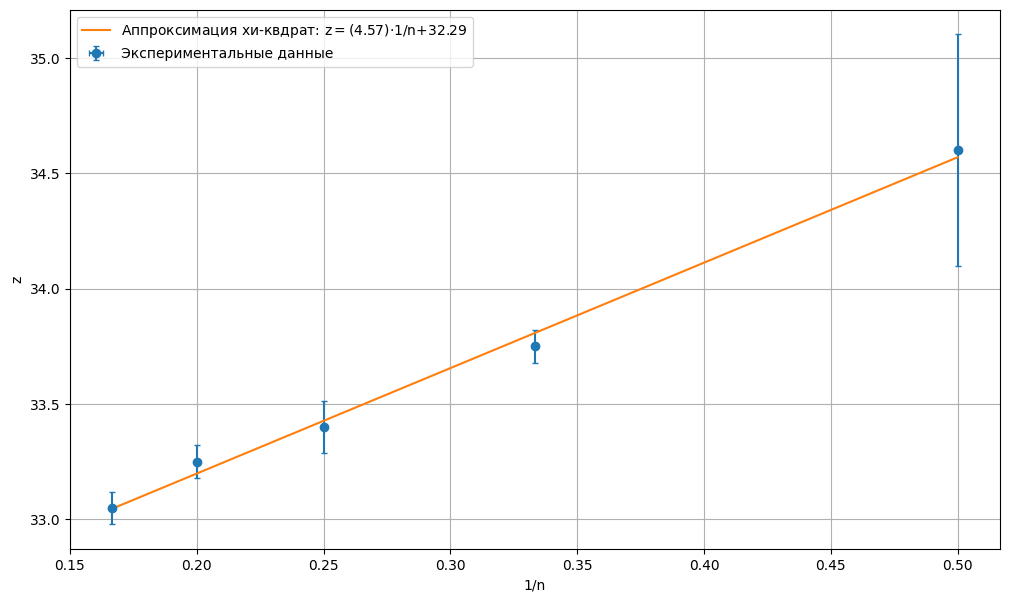
\includegraphics[width=\linewidth]{pic/A}
        \caption{График зависимость координаты минимума от номера}
        \label{fig:5}
    \end{figure}

    \begin{figure}[h!]
        \centering
        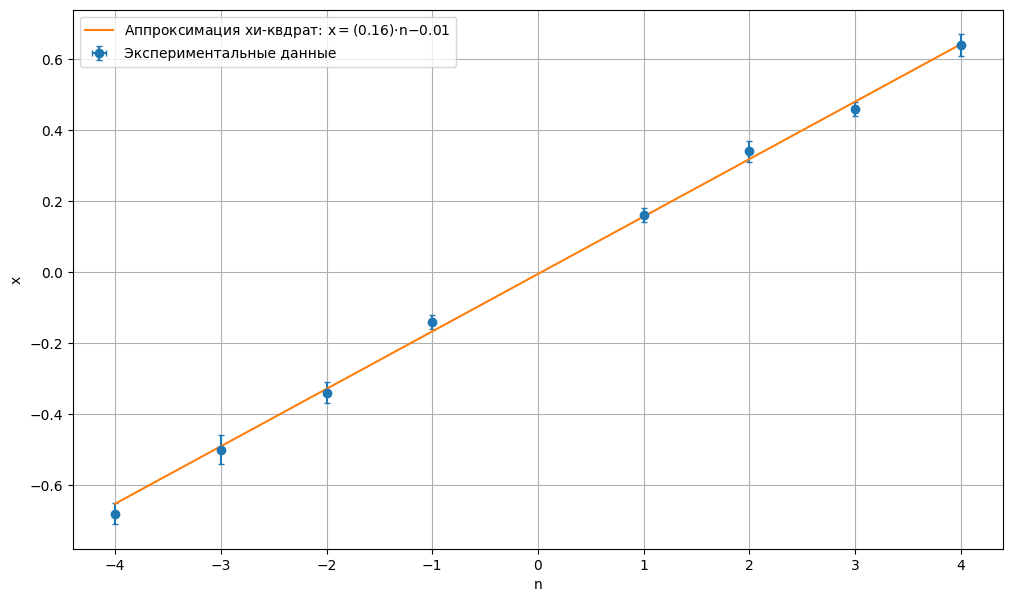
\includegraphics[width=\linewidth]{pic/B}
        \caption{График зависимости координаты минимума от номера}
        \label{fig:6}
    \end{figure}
\end{document}